%%spell
The decay \btodsphi proceeds via the annihilation of a the constituent quarks in the \Bp meson into
a virtual \Wp boson, as shown in \Fig{fig:dsphi:feyn}.
These types of decays are rare in the SM due to the magnitude of $|\V{ub}|$ (see \Eq{eq:th:vub});
in fact, no fully hadronic decays proceeding via annihilation have yet been observed.

Branching fraction predictions for \btodsphi are in the range (1--7)$\e{-7}$ in the SM
\cite{Zou:2009zza,Mohanta:2002wf,PhysRevD.76.057701,Lu:2001yz}

As discussed in \Sec{sec:th:bsm:man}, there is much interest in t



In the SM the decay is mediated by a \Wp gauge boson.

\begin{figure}
  \begin{center}
    %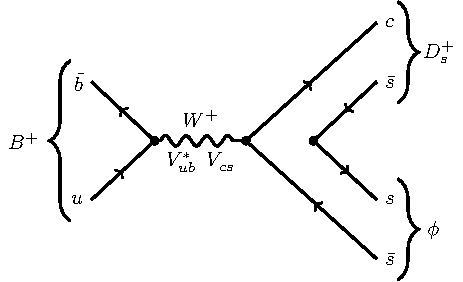
\includegraphics[width=0.48\textwidth]{feynman_dsphi_sm}
    %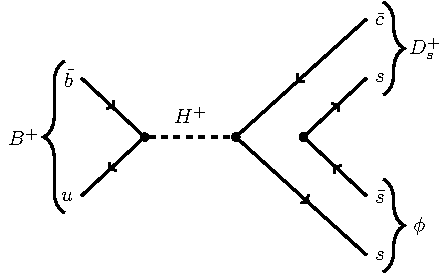
\includegraphics[width=0.48\textwidth]{feynman_dsphi_susy}
    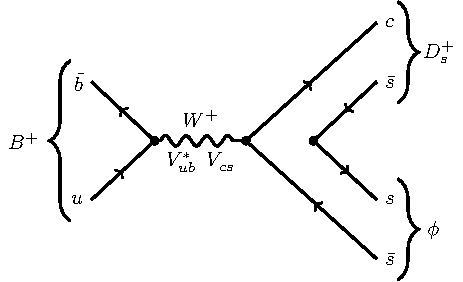
\includegraphics[scale=1]{feynman_dsphi_sm}
    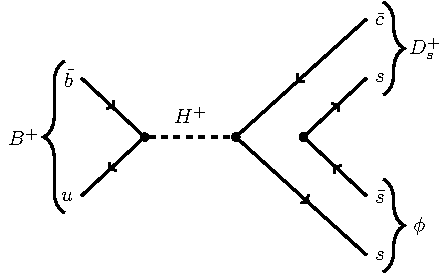
\includegraphics[scale=1]{feynman_dsphi_susy}
    \caption{\small
      A Feynman diagram for the decay \btodsphi being mediated by a
      (left) \Wp in the SM, and
      (right) $H^+$ in SUSY.
    }
    \label{fig:dsphi:feyn}
  \end{center}
\end{figure}


























In theory say that there is no longer a discrepancy (1407.1320).
\cite{PDG2012}
